\subsection{Robot Design}
\label{subsec:robotdesign}

\begin{figure} [ht]
  \centering
  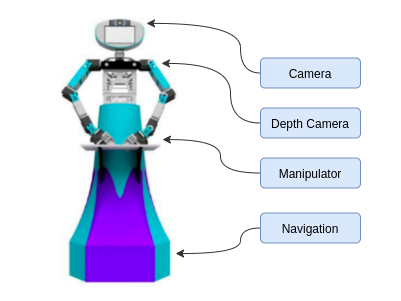
\includegraphics[width=0.4\textwidth]{images/robot-design.png}
  \caption{Diagram of the Dienen robot design.}
  \label{fig:robotdesign}
\end{figure}

The robot that will be used in this research is the Dienen robot which is a continuation of the IRIS robot \citep{dikairono2020}\citep{zanuar2019} with the addition of the ICHIRO robot \citep{muhtadin2019} design at the top of the robot.
A design like this is generally known as a mobile humanoid robot design \citep{mohamed2012},
  which is a combined design between a mobile robot and a humanoid robot.
As shown in Figure \ref{fig:robotdesign},
  the lower part of the robot resembles a mobile robot with three omnidirectional wheels driving which allows the robot to move in a holonomic way \citep{oliveira2008},
  while the upper part of the robot resembles a humanoid robot consisting of a body, head, and arms.
With the use of this mobile humanoid robot design,
  it is expected that users can experience better social interaction with the robot because it has a human-like appearance \citep{rossi2018} while making it easier for the robot to navigate in various places.

The Dienen robot is equipped with several sensors such as an IMU (inertial measurement unit) sensor to determine the orientation of the robot,
  rotary encoder sensors to perform odometry calculations from the robot,
  distance sensors to detect the presence of other objects around the robot,
  a camera sensor in the head to capture images,
  and a depth camera sensor that can be used to do mapping of a room.
In addition, this robot is also equipped with two manipulator arms that can be adjusted in various positions and orientations \citep{iqbal2012}.
With the presence of these sensors and actuators,
  it is expected that the robot will be able to carry out socially assistive actions in accordance with the data obtained from existing sensors.
